\section{Discussion of The Battery Modeling Results}
The results from the power analyzer have been satisfactory and the robustness of the power analyzer architecture allows for the simulation of various BMS tests, such as low battery voltage, high battery voltage protection, and soc estimation.
Batteries can be imbalanced for testing different battery balancing algorithms in the battery pack module by passing different initial SoC values. In the practical sense, low and high battery voltage testing takes tons of time with batteries. Achieving fast charging and discharging with the batteries needs a high sink/source current, which could be a limitation in many instruments. Thanks to the PowerAnalyzer, it allows emulating fast charging and discharging of batteries by adding some bias current(only added in the script) with the actual current that is flowing in the battery emulator. The actual battery emulator does not know anything it is not smart enough to realize what is going on with the current flowing in the system. On contrary, the script can emulate this behavior and set a new terminal voltage to each channel of the battery emulator, every time the PowerAnalyzer sample the current flowing in the battery emulator.

The following code, snippet illustrates the biased current simulation. "$currents = self.batEmulator.BateryEmulatorCellCurrent$" will fetch the actual current that is flowing in the battery emulator; for the "$currents$" array the "$ibattBias$" biased current is added and calculated as new open circuit voltage "$batEmulator.batteryEmulatorVoltageSet(cellNo=i,cellVoltage=VOC)$", and SoC is the updated, updated soc can help to determine the new open circuit voltage(VOC) and VOC set to the battery emulator as terminal voltage(each channel respectively).
\begin{lstlisting}[language=Python, caption=Emulating Sudo BiasCurrent in the PowerAnalyzer ]
    def batVoltageSOC(self):
        batVoltSOC =dict()
        currents = self.batEmulator.BateryEmulatorCellCurrent
        
        biasedCurrent = []
        # print(f'Current that flowinf in Chroma {currents}')
        
        #add the sudo bias current 
        for i in range(0,len(self.SOC0)):
            biasedCurrent.append(currents[i]+self.ibattBias)
                
        for i in range(0,len(self.SOC0)):
            [batVlot,VOC] = self.Batt[i].battVoltage(biasedCurrent[i])
            batVoltSOC[batVlot] = self.Batt[i].CoulombSOC
            self.batEmulator.batteryEmulatorVoltageSet(cellNo=i,
                                    cellVoltage=VOC)
            
        return batVoltSOC
\end{lstlisting}

\begin{figure}[h]
	\centering
	\subfigure[Battery Voltage Vs SOC @Charging]{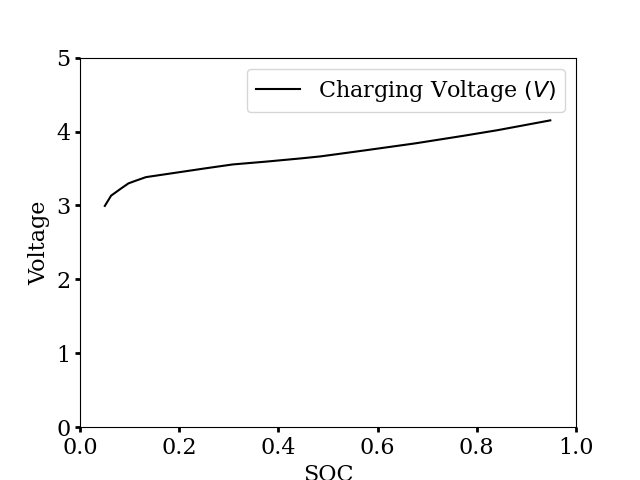
\includegraphics[scale=.4]{Chap06/Figures/PowerAnalyzerResults/Batt_Charging_Voltage_SOC.png}}\label{fig:Batt_Charging_Voltage_SOC}
	\qquad
	\subfigure[Battery Voltage Vs SOC @Discharging]{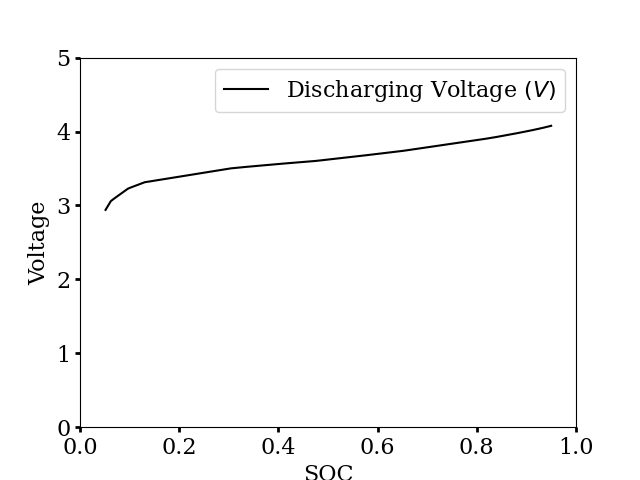
\includegraphics[scale=.4]{Chap06/Figures/PowerAnalyzerResults/Batt_Discharging_Voltage_SOC.png}}\label{fig:Batt_Discharging_Voltage_SOC}
	\qquad
	\subfigure[Battery Voltage Vs Cycles @Charging and Discharging]{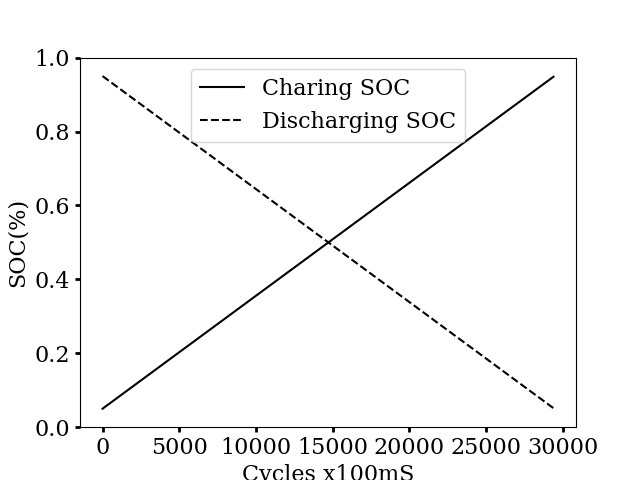
\includegraphics[scale=.4]{Chap06/Figures/PowerAnalyzerResults/Batt_Discharging_Charging_SOC_Cycles.png}}\label{fig:Batt_Discharging_Charging_SOC_Cycles}
	\qquad
	\subfigure[Battery SOC Vs Cycles @Charging and Discharging]{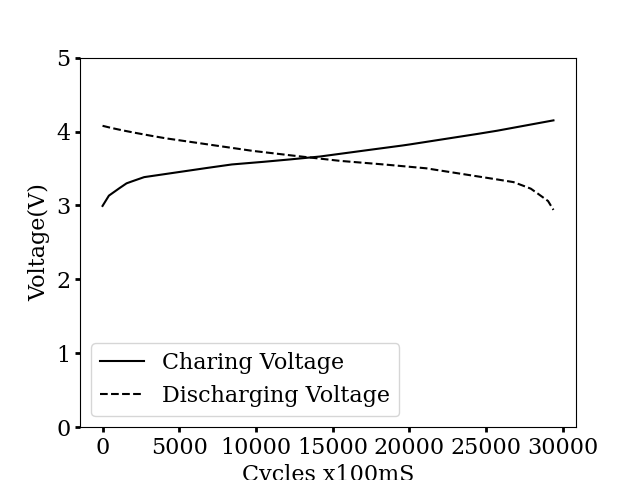
\includegraphics[scale=.4]{Chap06/Figures/PowerAnalyzerResults/Batt_Discharging_Charging_Voltage_Cycles.png}}\label{fig:Batt_Discharging_Charging_Voltage_Cycles}
	\caption{Single Battery Modeling Characteristics with PowerAnalyzer }\label{fig:Single_Batt_Modeling_Results}
\end{figure}

\begin{figure}[h]
	\centering
	\subfigure[Battery Pack Voltages Vs Cycles @Charging (same SOC)]{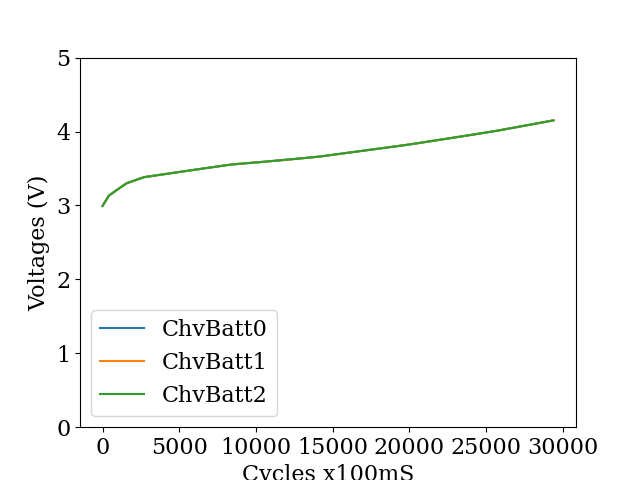
\includegraphics[scale=.4]{Chap06/Figures/PowerAnalyzerResults/Batt_Pack_Charging_Voltage_Cycles.png}}\label{fig:Batt_Pack_Charging_Voltage_Cycles}
	\qquad
	\subfigure[Battery Pack Voltages Vs Cycles @Discharging (same SOC)]{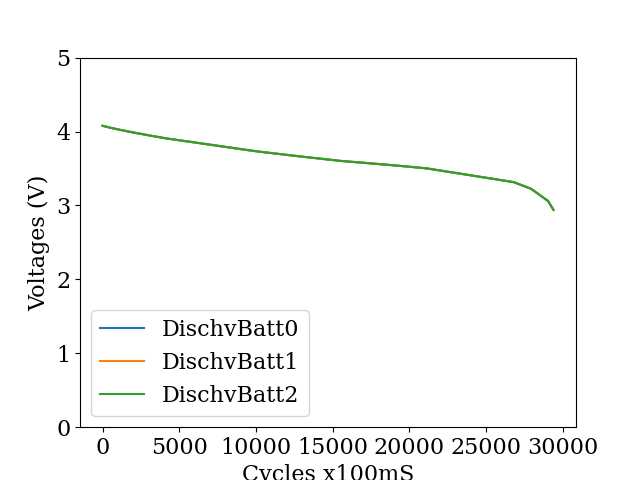
\includegraphics[scale=.4]{Chap06/Figures/PowerAnalyzerResults/Batt_Pack_Discharging_Voltage_Cycles.png}}\label{fig:Batt_Pack_Discharging_Voltage_Cycles}
	\qquad
	\subfigure[Battery Pack SOCs Vs Cycles @Charging and Discharging (same SOC)]{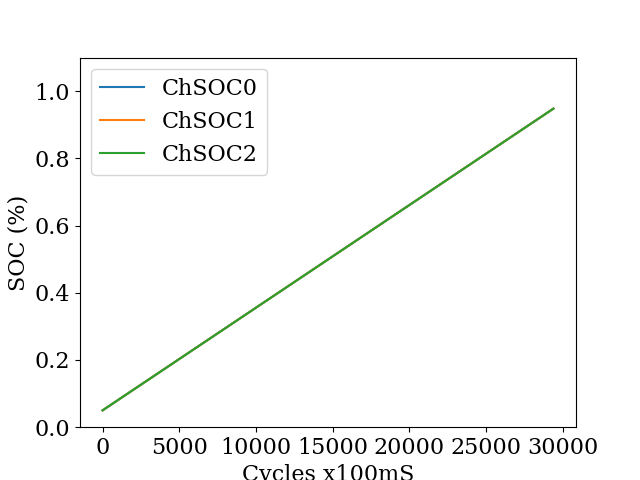
\includegraphics[scale=.4]{Chap06/Figures/PowerAnalyzerResults/Batt_Pack_Charging_SOC_Cycles.png}}\label{fig:Batt_Pack_Charging_SOC_Cycles}
	\qquad
	\subfigure[Battery Pack SOCs Vs Cycles @Charging and Discharging (same SOC)]{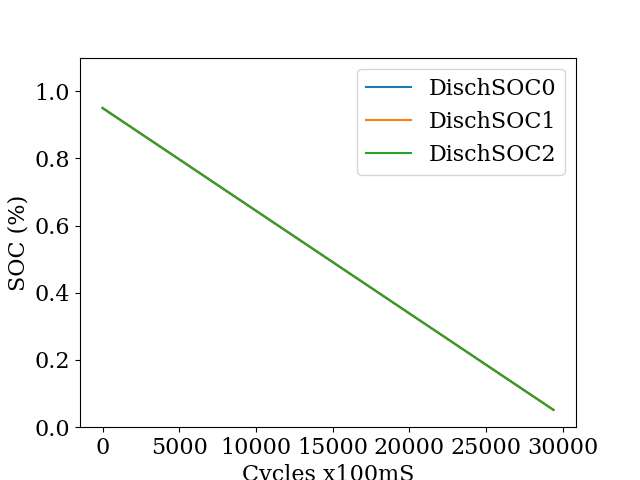
\includegraphics[scale=.4]{Chap06/Figures/PowerAnalyzerResults/Batt_Pack_Discharging_SOC_Cycles.png}}\label{fig:Batt_Pack_Discharging_SOC_Cycles}
	\qquad
	\subfigure[Battery Pack SOCs Vs Cycles @Charging(Different SOC)]{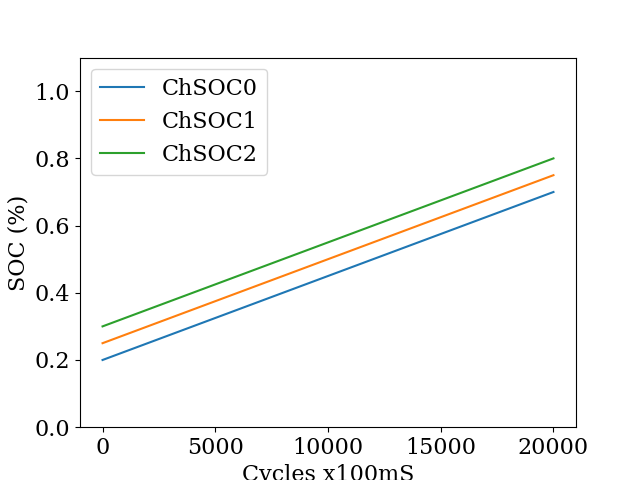
\includegraphics[scale=.4]{Chap06/Figures/PowerAnalyzerResults/Batt_Pack_Diff_SOC_Charging_SOC_Cycles.png}}\label{fig:Batt_Pack_Diff_SOC_Charging_SOC_Cycles}
	\qquad
	\subfigure[Battery Pack SOCs Vs Cycles @Charging(Different SOC)]{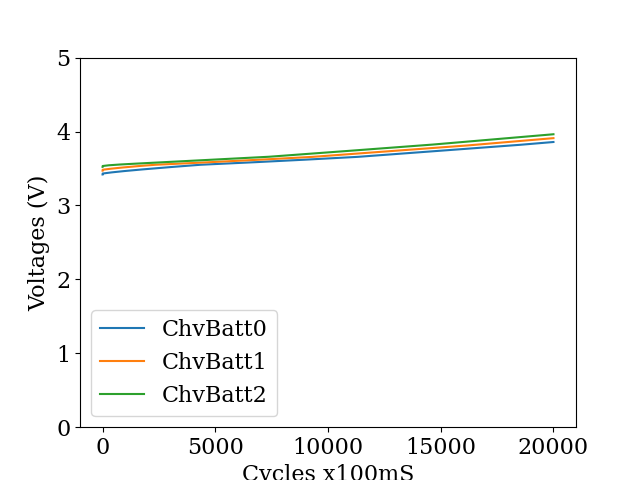
\includegraphics[scale=.4]{Chap06/Figures/PowerAnalyzerResults/Batt_Pack_Diff_SOC_Charging_Voltage_Cycles.png}}\label{fig:Batt_Pack_Diff_SOC_Charging_Voltage_Cycles}
	\caption{Battery Pack Modeling Characteristics with PowerAnalyzer(3 Cells) } \label{fig:Batt_Pack_Modeling_Results}
\end{figure}

The results in \ref{fig:Single_Batt_Modeling_Results} will enrich the battery modeling and power analyzer implementation, the data shown in the figure  \ref{fig:Single_Batt_Modeling_Results} will collect for one single battery with a one-time constant model. The data has been collected for one single battery from full charge to discharge, soc is from $5\%$ to $95\%$, and vice versa. The obtained results of battery voltage Vs SoC must match with the Voltage Soc curve provided by the manufacturer.
The charging voltage and soc \ref{fig:Single_Batt_Modeling_Results}(a) (discharging \ref{fig:Single_Batt_Modeling_Results}(b)) of the battery impressively match the results provided by the manufacturer in the voltage SoC graph \ref{fig:Battery_OCV_Vs_Soc}. 
Undoubtedly the battery modeling \ref{fig:Single_Batt_Modeling_Results} results match the OCV curve of the battery \ref{fig:Single_Batt_Modeling_Results}(a) and \ref{fig:Single_Batt_Modeling_Results}(b), yet it is very important to consider the symmetry of the OCV curve during charging and discharging Figure \ref{fig:Single_Batt_Modeling_Results}(c) and \ref{fig:Single_Batt_Modeling_Results}(d). The charging and discharging of curves of the battery are symmetry about $47\%$ of the SoC, which is a good sign for an estimate of the battery soc both at charging and discharging.
Figure \ref{fig:Single_Batt_Modeling_Results}(c) and \ref{fig:Single_Batt_Modeling_Results}(d)  plotted battery voltage and SoC vs cycles, several consecutive sampling times between the measurements are cycles. The sampling $dt$ time in this project has used multiples of 100mS. Nevertheless, $dt$ is the independent choice for the user which again depends on the application.

The target of the battery modeling is to build the battery pack with sophisticated control over it for BMS applications. Results in Figure \ref{fig:Batt_Pack_Modeling_Results} achieved such a target, I have implemented for 8 batteries (The Figures show only 3 battery results, to avoid clumsiness in the graphs).
The battery pack results are pretty much the same as results collected for a single battery Figures \ref{fig:Batt_Pack_Modeling_Results}(a) and \ref{fig:Batt_Pack_Modeling_Results}(d) show results for 8 batteries simulated with the same SOC assigned for all batteries. Thanks to the power analyzer, which will allow several battery tests for instance keep different socs and perform battery balancing, battery low and high voltage cut off. Figures \ref{fig:Batt_Pack_Modeling_Results}(e) and \ref{fig:Batt_Pack_Modeling_Results}(f) shows one such example of keeping different socs charging the batteries.